\documentclass[11pt,letterpaper]{article}

\usepackage[utf8]{inputenc}
\usepackage[T1]{fontenc}
\usepackage{lmodern}
\usepackage[spanish]{babel}
\usepackage[margin=2.5cm]{geometry}
\usepackage{graphicx}
\usepackage{xcolor}
\usepackage{listings}
\usepackage{fancyhdr}
\usepackage{hyperref}

\hypersetup{colorlinks=true, urlcolor=blue}

\pagestyle{fancy}
\fancyhf{}
\fancyhead[L]{ICN-292 --- Sistemas de Información para la Gestión}
\fancyhead[R]{Laboratorio 4 | 2026-2}
\fancyfoot[C]{\thepage}

\lstset{
    language=SQL,
    basicstyle=\ttfamily\small,
    keywordstyle=\color{blue}\bfseries,
    stringstyle=\color{orange!80!black},
    commentstyle=\color{gray},
    morekeywords={LIMIT, BETWEEN, ENUM, AUTO_INCREMENT, IF, EXISTS},
    frame=single,
    breaklines=true,
    columns=fullflexible,
    keepspaces=true,
    showstringspaces=false,
    literate={á}{{\'a}}1 {é}{{\'e}}1 {í}{{\'i}}1 {ó}{{\'o}}1 {ú}{{\'u}}1
             {Á}{{\'A}}1 {ñ}{{\~n}}1
}

\begin{document}

% ------------------------------------------------------------
% Portada
% ------------------------------------------------------------
\begin{titlepage}
    \centering
    
\includegraphics[width=0.22\textwidth]{img/logo_usm.png}\par
    \vspace{0.8cm}
    {\large\textsc{Universidad Técnica Federico Santa María}\par}
    \vspace{0.2cm}
    ICN-292 --- Sistemas de Información para la Gestión \quad $|$ \quad Semestre 2026-2\par
    \vspace{3cm}
    \rule{0.75\textwidth}{0.6pt}\par
    \vspace{0.6cm}
    {\LARGE\textbf{Laboratorio 4}\par}
    \vspace{0.3cm}
    Consultas SQL sobre la base de Austral Editores\par
    \vspace{0.6cm}
    \rule{0.75\textwidth}{0.6pt}\par
    \vfill
    \raggedright
    \textbf{Alumno:} Claudio Vera Ávila\par\vspace{0.2cm}
    \textbf{Rol:} 202104575-9\par\vspace{0.2cm}
    \textbf{Paralelo:} 100\par\vspace{0.2cm}
    \textbf{Fecha de entrega:} 8 de noviembre de 2026\par\vspace{0.2cm}
    \textbf{Repositorio:} \url{https://github.com/claudioveravila/ICN292-Lab4-Vera-Claudio}\par
    \vspace{1cm}
\end{titlepage}

% ------------------------------------------------------------
% Consultas
% ------------------------------------------------------------
\clearpage
\noindent\begin{minipage}{\linewidth}
\section*{Consulta 1}

Muestre el nombre y el género de los autores cuyo país no es Chile, incluyendo a quien no tiene país registrado, ordenados por nombre.

\begin{lstlisting}
SELECT nombre, genero
FROM   autores
WHERE  pais <> 'Chile' OR pais IS NULL
ORDER BY nombre;
\end{lstlisting}

\begin{center}
    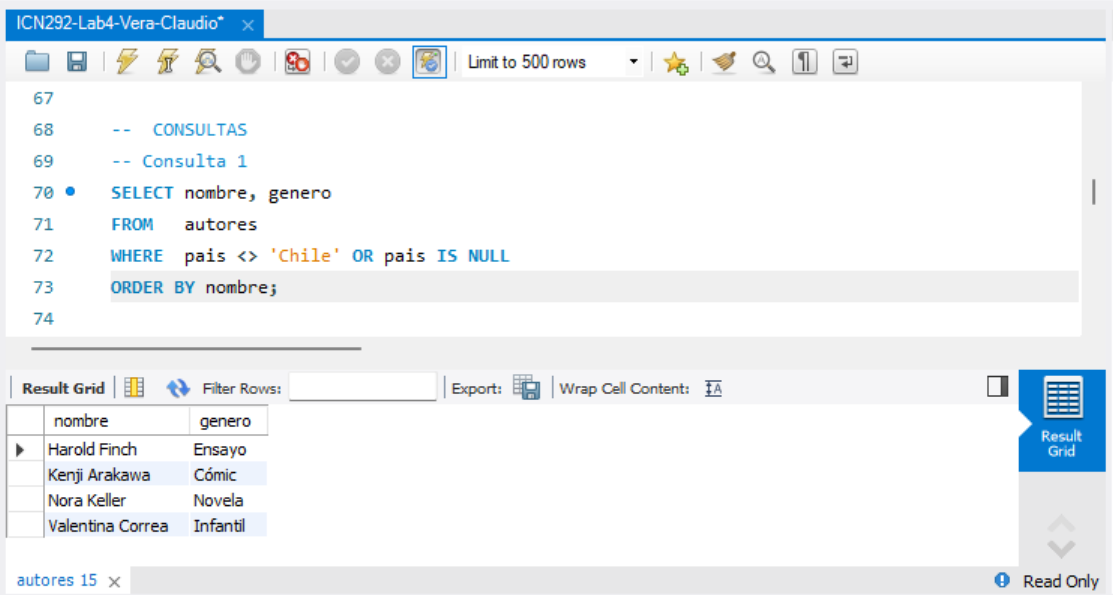
\includegraphics[width=0.72\linewidth]{img/c1.png}
\end{center}

Con solo \texttt{pais <> 'Chile'} Kenji Arakawa no aparece, porque su país está en NULL y comparar un NULL no da verdadero sino desconocido, así que hay que agregar \texttt{OR pais IS NULL} para que salga.
\end{minipage}
\par\vspace{0.6cm}

\noindent\begin{minipage}{\linewidth}
\section*{Consulta 2}

Liste el título y las páginas de los libros que tienen entre 190 y 220 páginas, incluidos los dos valores, de menor a mayor número de páginas.

\begin{lstlisting}
SELECT titulo, paginas
FROM   libros
WHERE  paginas BETWEEN 190 AND 220
ORDER BY paginas;
\end{lstlisting}

\begin{center}
    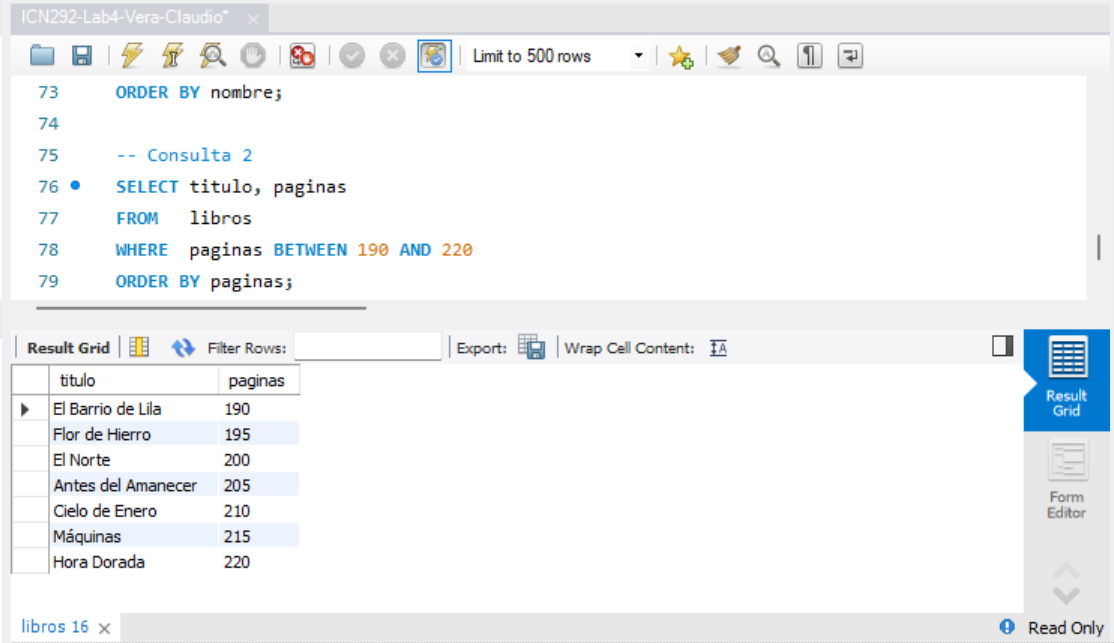
\includegraphics[width=0.72\linewidth]{img/c2.png}
\end{center}
\end{minipage}
\par\vspace{0.6cm}

\noindent\begin{minipage}{\linewidth}
\section*{Consulta 3}

Entregue una sola fila con el número de libros del catálogo, la suma de ejemplares vendidos, el promedio de páginas, el año más antiguo y la mayor cantidad de ejemplares vendidos de un libro. Cada columna lleva un alias.

\begin{lstlisting}
SELECT COUNT(*)                  AS total_libros,
       SUM(ejemplares_vendidos)  AS total_ejemplares,
       AVG(paginas)              AS promedio_paginas,
       MIN(anio)                 AS anio_mas_antiguo,
       MAX(ejemplares_vendidos)  AS max_ejemplares
FROM   libros;
\end{lstlisting}

\begin{center}
    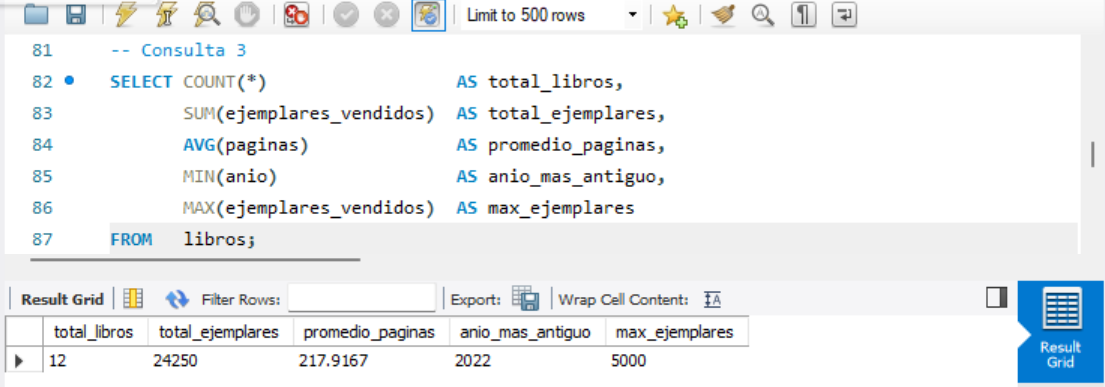
\includegraphics[width=0.72\linewidth]{img/c3.png}
\end{center}
\end{minipage}
\par\vspace{0.6cm}

\noindent\begin{minipage}{\linewidth}
\section*{Consulta 4}

Liste los géneros distintos de los autores, una vez cada uno, en orden alfabético.

\begin{lstlisting}
SELECT DISTINCT genero
FROM   autores
ORDER BY genero;
\end{lstlisting}

\begin{center}
    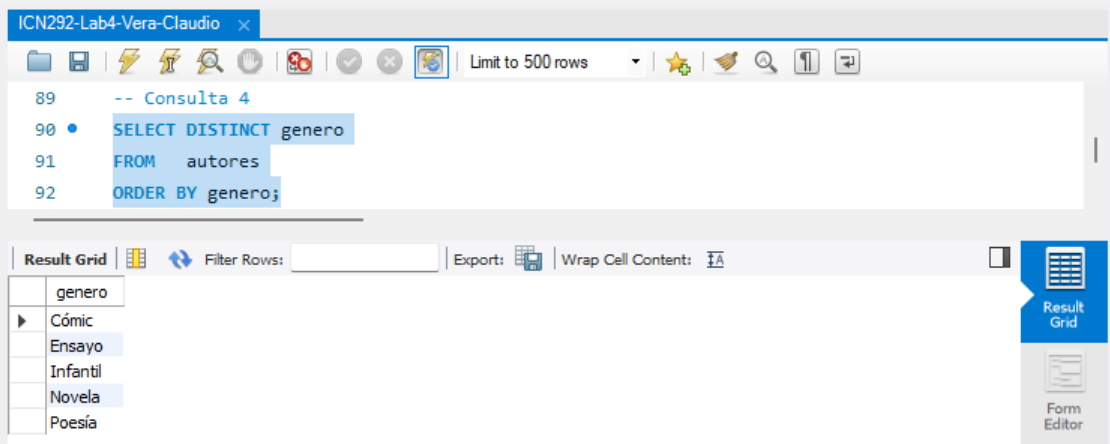
\includegraphics[width=0.72\linewidth]{img/c4.png}
\end{center}
\end{minipage}
\par\vspace{0.6cm}

\noindent\begin{minipage}{\linewidth}
\section*{Consulta 5}

Muestre el nombre de cada autor que tiene más de un libro publicado en 2024 y cuántos son. Ordene por nombre.

\begin{lstlisting}
SELECT   a.nombre, COUNT(*) AS libros_2024
FROM     autores a
JOIN     libros  l ON a.id_autor = l.id_autor
WHERE    l.anio = 2024
GROUP BY a.id_autor, a.nombre
HAVING   COUNT(*) > 1
ORDER BY a.nombre;
\end{lstlisting}

\begin{center}
    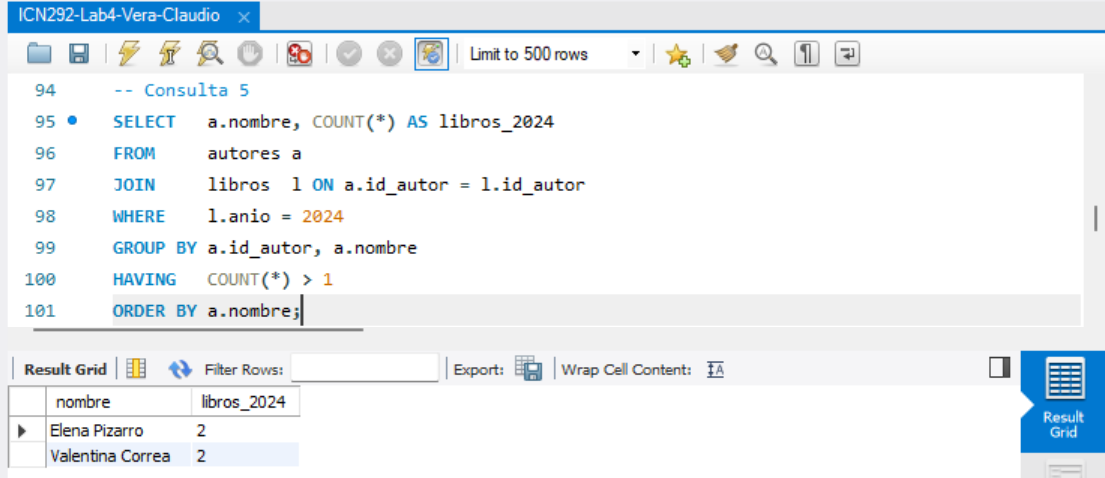
\includegraphics[width=0.72\linewidth]{img/c5.png}
\end{center}
\end{minipage}
\par\vspace{0.6cm}

\noindent\begin{minipage}{\linewidth}
\section*{Consulta 6}

Liste el título y los ejemplares vendidos de los libros de 2024 que superan los 2\,000 ejemplares, de mayor a menor. Muestre solo los tres primeros.

\begin{lstlisting}
SELECT titulo, ejemplares_vendidos
FROM   libros
WHERE  anio = 2024 AND ejemplares_vendidos > 2000
ORDER BY ejemplares_vendidos DESC
LIMIT 3;
\end{lstlisting}

\begin{center}
    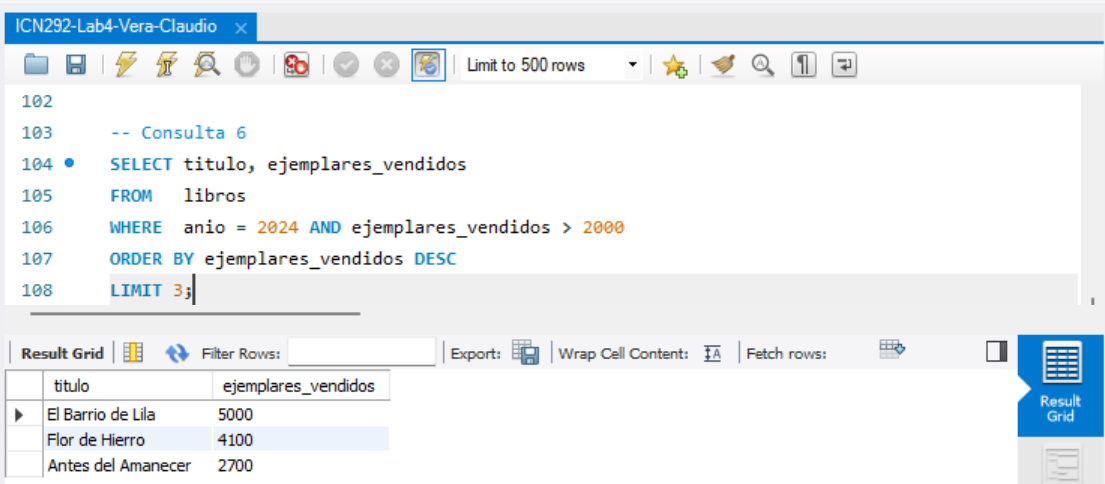
\includegraphics[width=0.72\linewidth]{img/c6.png}
\end{center}
\end{minipage}
\par\vspace{0.6cm}

\noindent\begin{minipage}{\linewidth}
\section*{Consulta 7}

Inserte el libro `Papel Mojado', de Rodrigo Bahamonde, con 260 páginas, 50 ejemplares vendidos y año 2024. Después elimínelo con un DELETE que filtre por título. Escriba un SELECT con ese mismo criterio antes del DELETE, para ver la fila que va a borrar, y otro después, para comprobar que ya no está.

\begin{lstlisting}
INSERT INTO libros (id_autor, titulo, paginas, ejemplares_vendidos, anio)
VALUES (3, 'Papel Mojado', 260, 50, 2024);

SELECT * FROM libros
WHERE  titulo = 'Papel Mojado' AND id_libro > 0;

DELETE FROM libros
WHERE  titulo = 'Papel Mojado' AND id_libro > 0;

SELECT * FROM libros
WHERE  titulo = 'Papel Mojado' AND id_libro > 0;
\end{lstlisting}

\begin{center}
    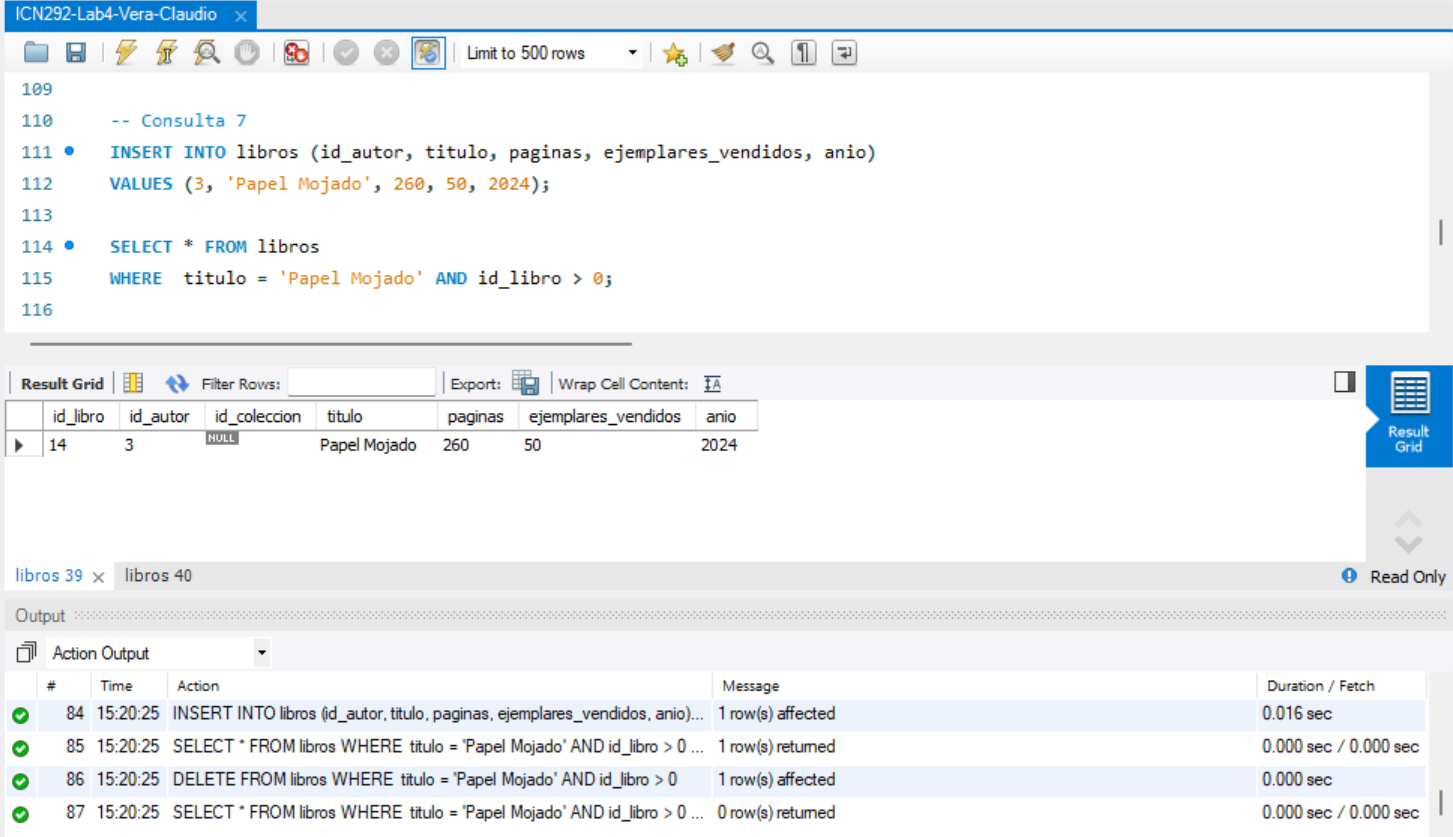
\includegraphics[width=0.72\linewidth]{img/c7_1.png}

    {\small\textit{Antes del DELETE: aparece la fila de Papel Mojado.}}
\end{center}
\end{minipage}
\par\vspace{0.6cm}

\noindent\begin{minipage}{\linewidth}
\begin{center}
    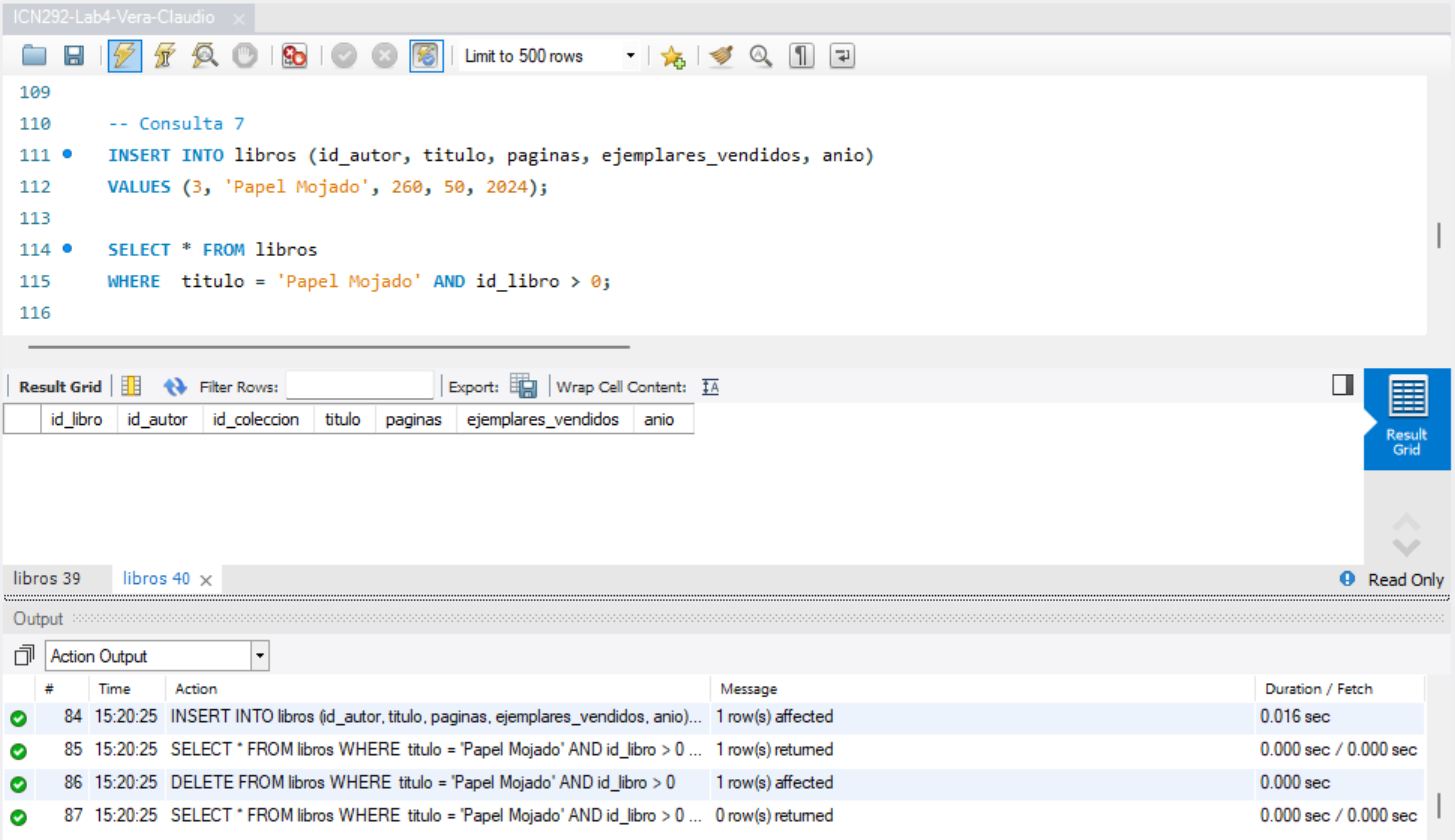
\includegraphics[width=0.72\linewidth]{img/c7_2.png}

    {\small\textit{Después del DELETE: el SELECT ya no devuelve nada.}}
\end{center}
\end{minipage}
\par\vspace{0.6cm}

\noindent\begin{minipage}{\linewidth}
\section*{Consulta 8}

Sume 100 ejemplares vendidos a `Cielo de Enero'. El UPDATE debe calcular el valor nuevo a partir del actual, no escribir el resultado a mano. Entregue tres capturas: el SELECT previo con el mismo WHERE, el UPDATE y el SELECT posterior.

\begin{lstlisting}
SELECT titulo, ejemplares_vendidos
FROM   libros
WHERE  id_libro = 1;

UPDATE libros
SET    ejemplares_vendidos = ejemplares_vendidos + 100
WHERE  id_libro = 1;

SELECT titulo, ejemplares_vendidos
FROM   libros
WHERE  id_libro = 1;
\end{lstlisting}

\begin{center}
    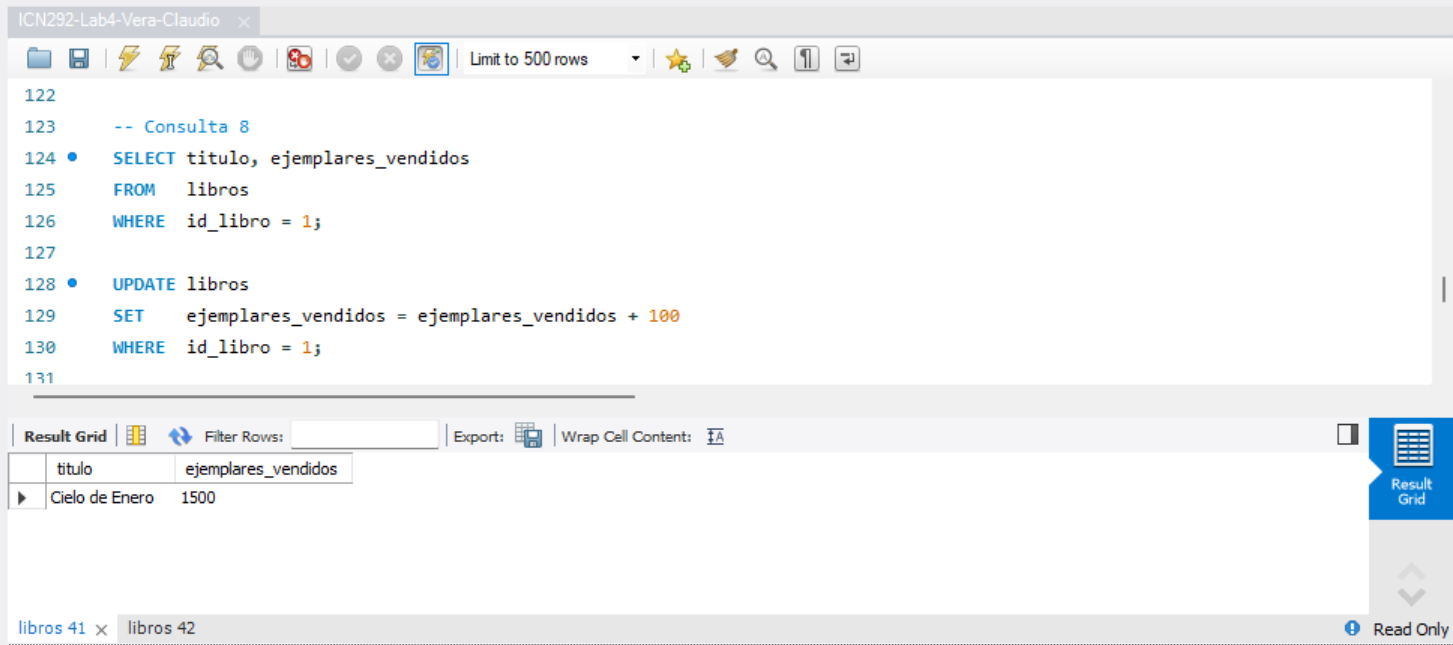
\includegraphics[width=0.72\linewidth]{img/c8_1.png}

    {\small\textit{SELECT antes del cambio: 1500 ejemplares.}}
\end{center}
\end{minipage}
\par\vspace{0.6cm}

\noindent\begin{minipage}{\linewidth}
\begin{center}
    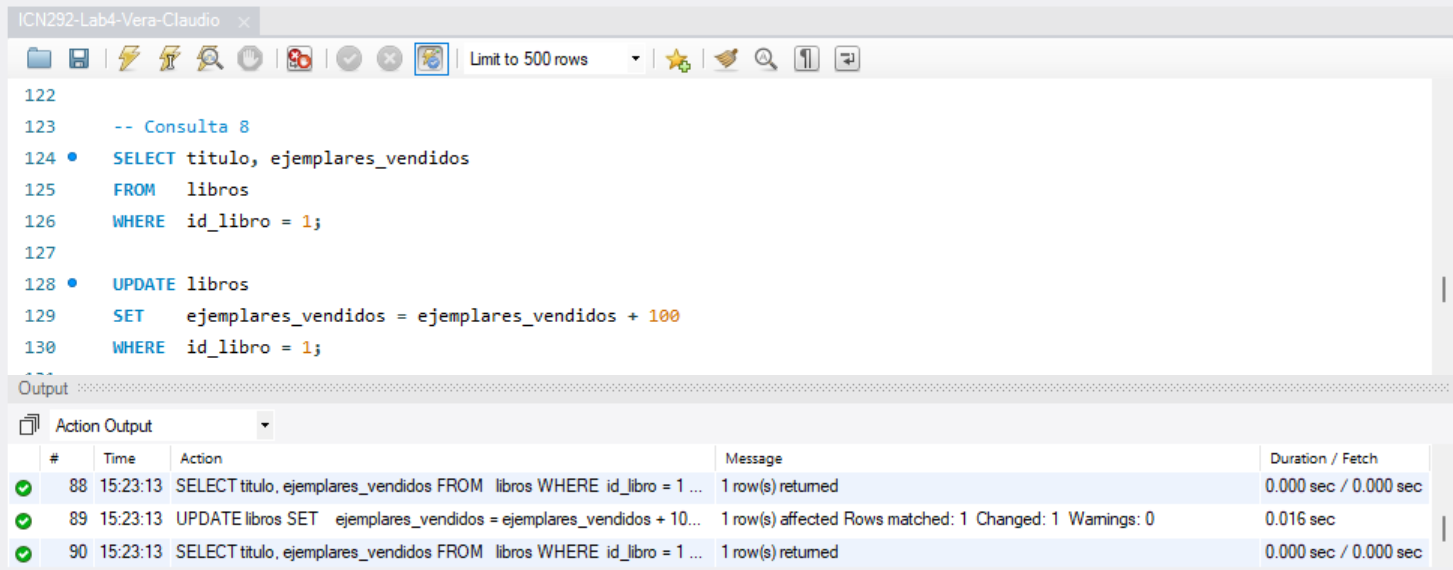
\includegraphics[width=0.72\linewidth]{img/c8_2.png}

    {\small\textit{El UPDATE ejecutado.}}
\end{center}
\end{minipage}
\par\vspace{0.6cm}

\noindent\begin{minipage}{\linewidth}
\begin{center}
    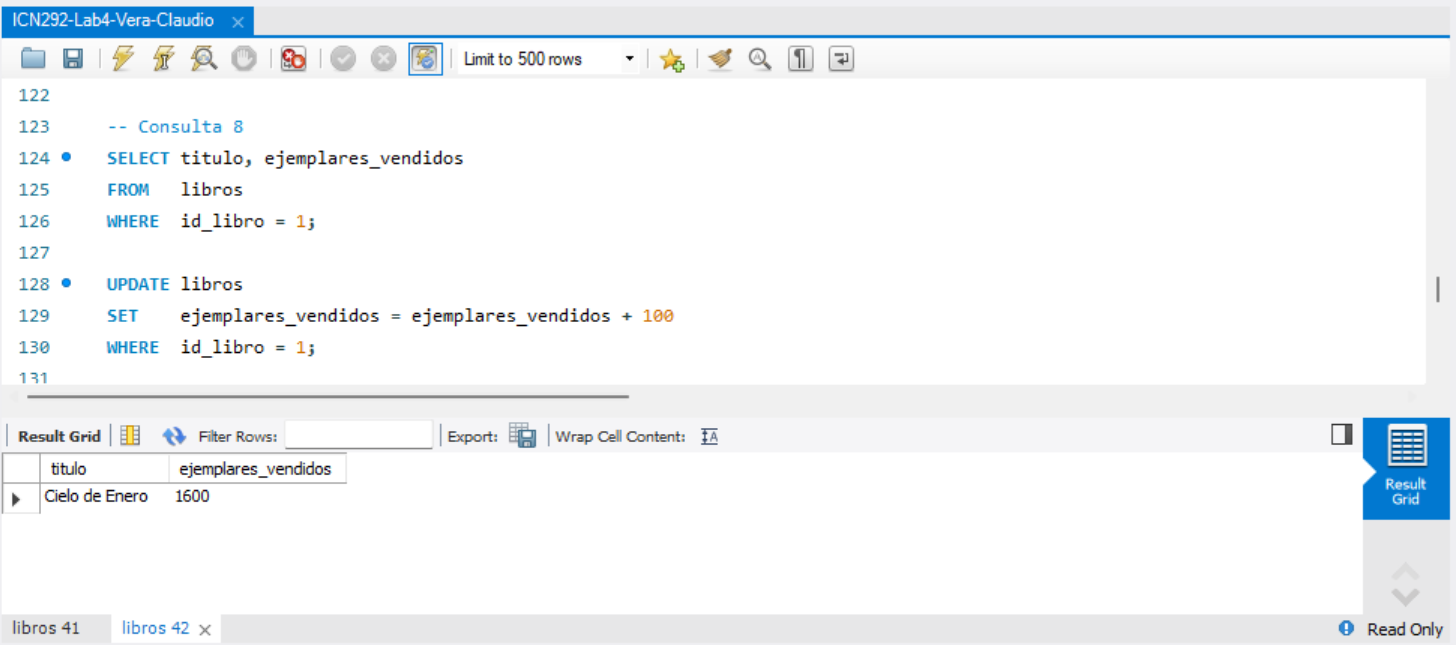
\includegraphics[width=0.72\linewidth]{img/c8_3.png}

    {\small\textit{SELECT después del cambio: 1600 ejemplares.}}
\end{center}
\end{minipage}
\par\vspace{0.6cm}

\noindent\begin{minipage}{\linewidth}
\section*{Consulta 9}

Liste el título de cada libro, el título de la colección a la que pertenece y la fecha de publicación de la colección. Un libro pertenece a una sola colección y una colección reúne varios libros. La fecha es un DATE. Cargue al menos dos colecciones en la tabla colecciones y asigne los doce libros.

\begin{lstlisting}
INSERT INTO colecciones (titulo, fecha_publicacion) VALUES
('Narrativa del Sur',  '2022-03-15'),
('Ideas y Versos',     '2022-09-01'),
('Pequeños Lectores',  '2023-04-20');

UPDATE libros SET id_coleccion = 1 WHERE id_libro IN (1, 2, 3, 11, 12);
UPDATE libros SET id_coleccion = 2 WHERE id_libro IN (4, 5, 6, 7);
UPDATE libros SET id_coleccion = 3 WHERE id_libro IN (8, 9, 10);

SELECT l.titulo AS libro,
       c.titulo AS coleccion,
       c.fecha_publicacion
FROM   libros      l
JOIN   colecciones c ON l.id_coleccion = c.id_coleccion
ORDER BY c.titulo, l.titulo;
\end{lstlisting}

\begin{center}
    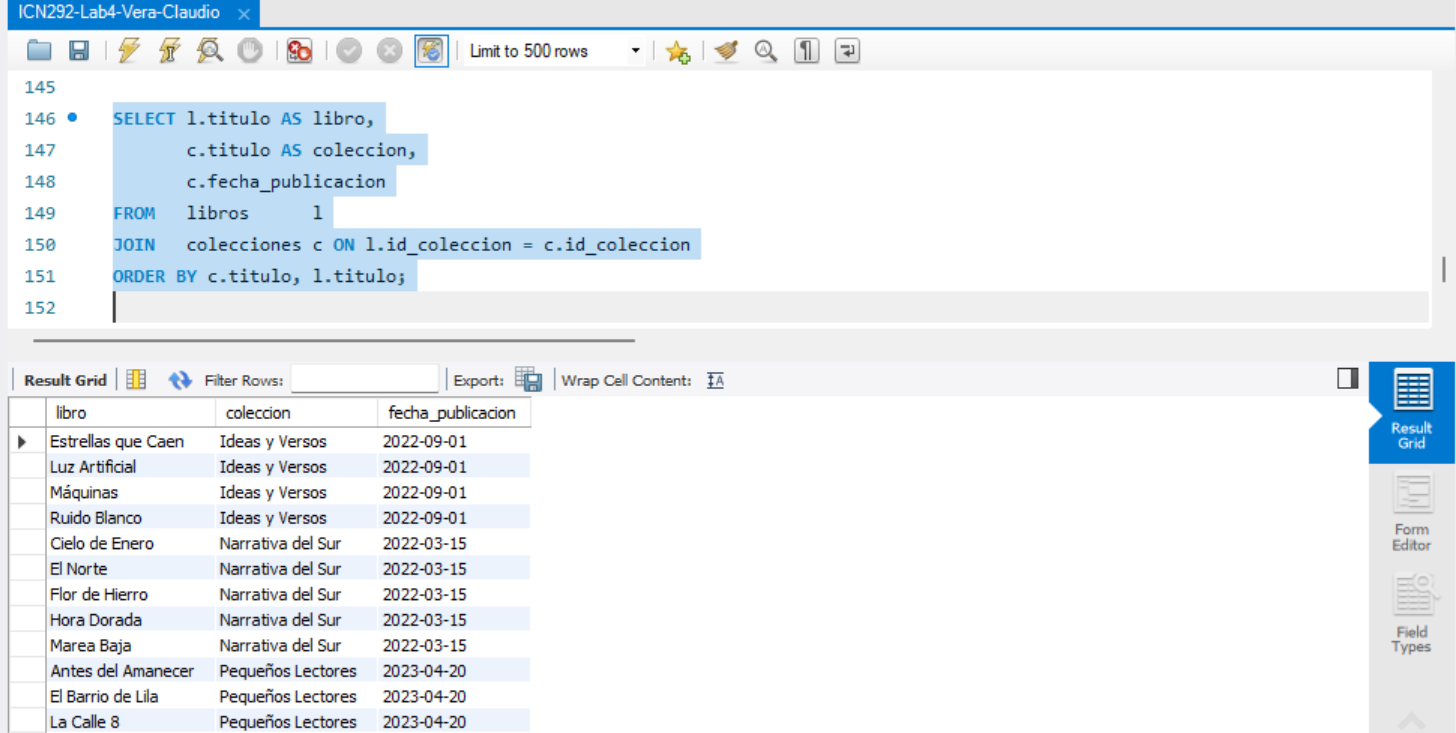
\includegraphics[width=0.72\linewidth]{img/c9.png}
\end{center}
\end{minipage}
\par\vspace{0.6cm}

\noindent\begin{minipage}{\linewidth}
\section*{Consulta 10}

Son dos sentencias. Primero liste los pagos hechos a los autores, con el nombre del autor, la fecha del pago y el monto; después muestre el total pagado a cada autor. La fecha es un DATE y el monto es un DECIMAL(10,2). Cargue al menos tres pagos en la tabla pagos, dos de ellos al mismo autor.

\begin{lstlisting}
INSERT INTO pagos (id_autor, fecha_pago, monto) VALUES
(1, '2026-03-31', 450000.00),
(1, '2026-06-30', 380500.50),
(4, '2026-06-30', 920000.00),
(5, '2026-07-15', 610250.75);

SELECT a.nombre, p.fecha_pago, p.monto
FROM   pagos   p
JOIN   autores a ON p.id_autor = a.id_autor
ORDER BY p.fecha_pago;

SELECT   a.nombre, SUM(p.monto) AS total_pagado
FROM     pagos   p
JOIN     autores a ON p.id_autor = a.id_autor
GROUP BY a.id_autor, a.nombre
ORDER BY a.nombre;
\end{lstlisting}

\begin{center}
    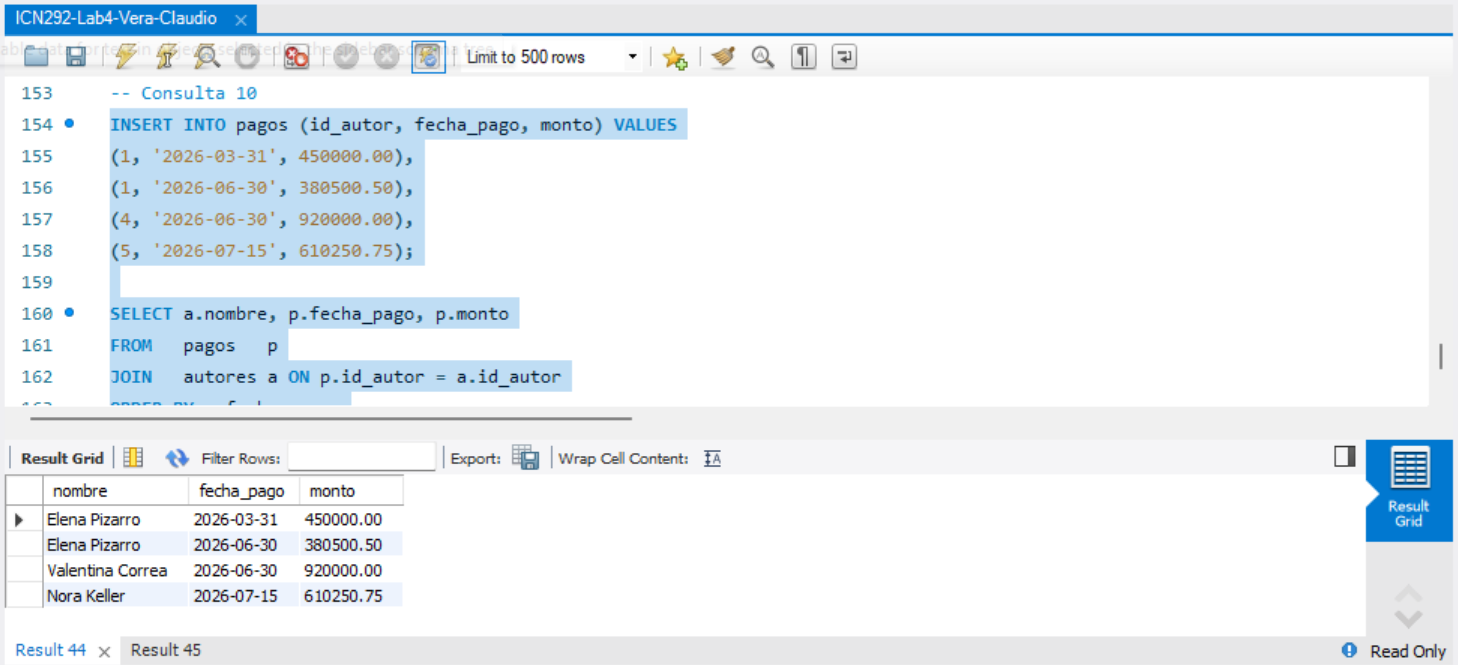
\includegraphics[width=0.72\linewidth]{img/c10_1.png}

    {\small\textit{Pagos hechos a los autores.}}
\end{center}
\end{minipage}
\par\vspace{0.6cm}

\noindent\begin{minipage}{\linewidth}
\begin{center}
    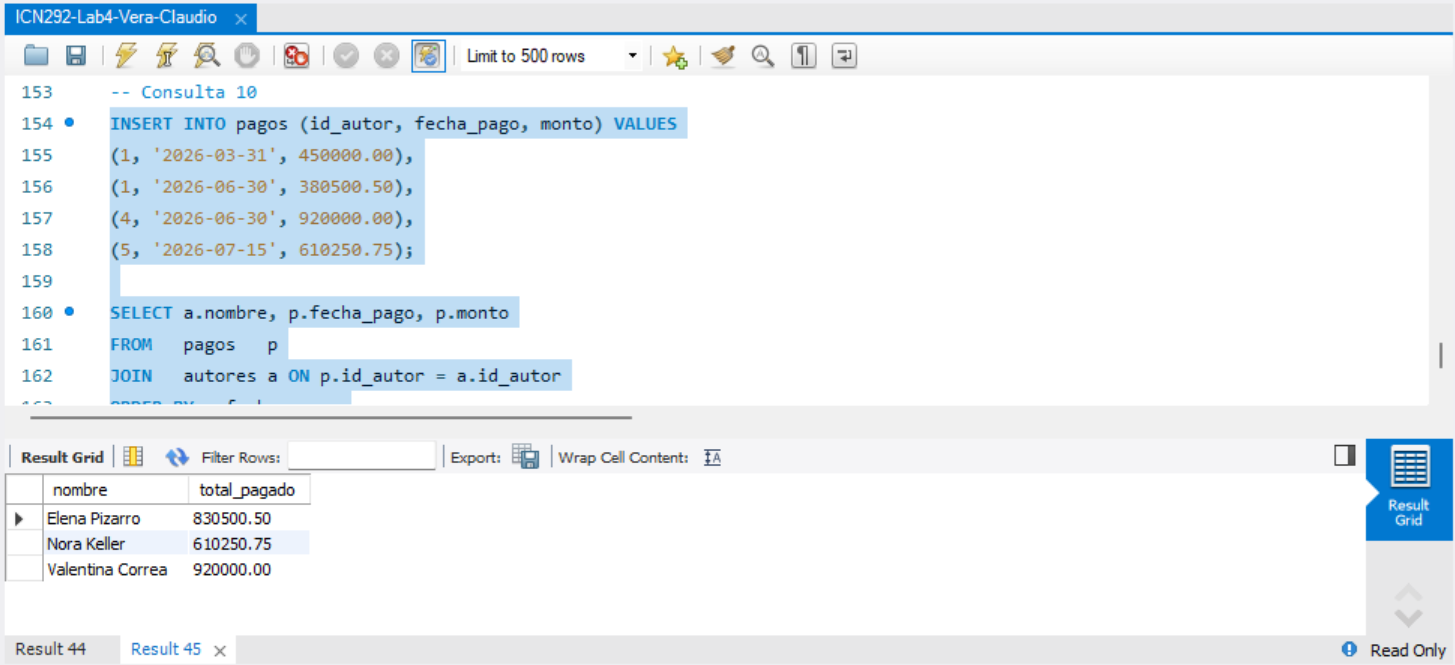
\includegraphics[width=0.72\linewidth]{img/c10_2.png}

    {\small\textit{Total pagado a cada autor.}}
\end{center}
\end{minipage}
\par\vspace{0.6cm}

\end{document}